\documentclass[a4paper; 11pt]{article}

% global includes
\usepackage[polish]{babel}
\usepackage[utf8]{inputenc}
\usepackage{polski}
\usepackage{courier} %times, kurier
\usepackage{amsmath}
\usepackage{amsfonts}
\usepackage{graphicx}
\usepackage{geometry}
\usepackage{indentfirst}
\usepackage{icomma}
\usepackage{booktabs}
\usepackage{paralist}
\usepackage{commath}
\usepackage{hyperref}
\usepackage{pgfplots}
\newgeometry{tmargin=2.3cm, lmargin=1.9cm, rmargin= 1.9cm, bmargin= 2.3cm}

\title{Badanie działania modelu Takagi-Sugeno dla różnych parametrów i~zbiorów danych}
\author{Marcin Kołodziej \and Jakub Sawicki}

\begin{document}
\renewcommand{\figurename}{Rys.}
\renewcommand{\tablename}{Tab.}
\renewcommand{\abstractname}{Abstrakt}

\maketitle

\section{Wstęp}

W~ramach projektu dokonano implementacji modelu rozmytego wnioskowania Takagi-Sugeno.
Reguły zaimplementowanego modelu opierają się na klastrach znalezionych przy
pomocy algorytmu rozmytego klastrowania --- Fuzzy C-Means.

Algorytmy zostały zaimplementowane w~języku programu MATLAB\@.

\subsection{Fuzzy C-Means}

Algorytm FCM dokonuje podziału grupy $N$ punktów wejściowych
$\mathbf{x}_j \in \mathbb{R}^n$ na $c$ klastrów o~prototypach
$\mathbf{v}_i \in \mathbb{R}^n$.
Przynależność punktu każdego z~klastrów określona jest za pomocą macierzy
przynależności $\mathbf{U}$, gdzie $u_{ij}$ określa przynależność punktu
$\mathbf{x}_j$ do klastra z~prototypem $\mathbf{v}_i$.
Macierz przynależności $\mathbf{U}$ spełniać musi następujące warunki
\begin{inparaenum}[ a)]
    \item $u_{ij} \in [0, 1]$
    \item $\forall{j \in [1, N]} \sum_{i=1}^c{u_{ij}} = 1$
    \item $\forall{i \in [1, c]} \sum_{j=1}^N{u_{ij}} > 0$.
\end{inparaenum}

Algorytm może być parametryzowany przez 
$c \in \mathbb{Z}$, $c > 1$ -- liczbę klastrów oraz 
$m \in \mathbb{R}$, $m > 1$ -- stopień ,,rozmycia''.

Miarą jakości rozwiązania jest $Q$ zdefiniowane przez
\begin{equation}
    Q = \sum\limits_{i=1}^c \sum\limits_{k=1}^N {u_{ik}^m \norm{\mathbf{x}_k - \mathbf{v}_i}^2} \text{ .}
    \label{eq:fcm:Q}
\end{equation}

Na początku generowana jest losowa macierz $\mathbf{U}$.
Zostaje ona znormalizowana aby spełniała wyżej określone warunki.

Następnie w~pętli wyliczane są kolejno prototypy korzystając z~macierzy
$\mathbf{U}$ z~poprzedniej iteracji:
\begin{equation}
    \mathbf{v}_i = \frac{
            \sum\limits_{k=1}^N {u_{ik}^m \mathbf{x}_k}
        }{% ------------------------------------
            \sum\limits_{k=1}^N {u_{ik}^m}
        } \text{ .}
    \label{eq:fcm:V}
\end{equation}
Na podstawie nowo wyliczonych prototypów liczona jest nowa macierz $\mathbf{U}$
\begin{equation}
    u_{st} = \frac{1}{\sum\limits_{j=1}^c {
        \left( \frac{
            \norm{\mathbf{x}_t - \mathbf{v}_s}}{
            \norm{\mathbf{x}_t - \mathbf{v}_j}} \right)^{
                \frac{2}{m - 1}}}} \text{ ,}
    \label{eq:fcm:U}
\end{equation}
gdzie norma $\norm{\cdot}$ zdefiniowana została jako norma Euklidesowa
$\norm{\mathbf{a}}^2 = \sum_{i=1}^n {a_i^2}$, dla $\mathbf{a} \in \mathbb{R}^n$.

Za warunek stopu przyjęty został
\begin{equation}
    \max_{\forall{i,j}}{\abs{u_{ij}^\text{aktualny} - u_{ij}^\text{poprzedni}}} < \varepsilon 
    \text{ , dla } \varepsilon > 0 \text{ .}
    \label{eq:fcm:stop}
\end{equation}


\subsection{Model Takagi-Sugeno}

Jest to model wnioskowania rozmytego oparty na regułach postaci
\begin{equation}
    \left\{ \texttt{ if } \mathbf{x} \texttt{ is } B_i \texttt{ then } f_i \right\}_{i~= 1,\dots,c} \text{ ,}
    \label{eq:ts:rules-text}
\end{equation}
gdzie
$B_i : \mathbb{R}^n \rightarrow [0, 1]$ -- funkcja przynależności $\mathbf{x}$ do reguły $i$ oraz
$f_i : \mathbb{R}^n \rightarrow \mathbb{R}$ -- funkcja przyporządkowana 
    $\mathbb{B}_i$, liniowa ze względu na parametry.

Zapisując \eqref{eq:ts:rules-text} w~bardziej sformalizowany sposób otrzymuje się
\begin{equation}
    \texttt{ if } \mathbf{x} \cdot A_i \texttt{ then } \hat{y}_i = L_i(\mathbf{x}) = a_{i0} + a_{i1} x_1 + \dots + a_{in} x_n =
    \begin{bmatrix}
        a_{i0} \\ a_{i1} \\ \vdots \\ a_{in}
    \end{bmatrix}^T
    \begin{bmatrix}
        1 \\ x_1 \\ \vdots \\ x_n
    \end{bmatrix} = \mathbf{a}_i^T \mathbf{z} \text{ .}
    \label{eq:ts:rules}
\end{equation}

Miara przynależności $A_i$ zdefiniowana jest analogicznie do \eqref{eq:fcm:U}
\begin{equation}
    A_i(\mathbf{x}) = \frac{1}{\sum\limits_{j=1}^c {
        \left( \frac{
            \norm{\mathbf{x} - \mathbf{v}_i}}{
            \norm{\mathbf{x} - \mathbf{v}_j}} \right)^{
                \frac{2}{m - 1}}}} \text{ .}
    \label{eq:ts:B}
\end{equation}

Dzięki temu, że $A_i(\mathbf{x}) \in \mathbb{R}$ możliwe jest następujące przekształcenie:
\begin{equation}
    \hat{y} = 
    \sum\limits_{i=1}^c {A_i(\mathbf{x}) L_i(\mathbf{x})} =
    \sum\limits_{i=1}^c {A_i(\mathbf{x}) \mathbf{a}_i^T \mathbf{z}} =
    \sum\limits_{i=1}^c \mathbf{a}_i^T \underbrace{A_i(\mathbf{x}) \mathbf{z}}_{\mathbf{g}_i(\mathbf{x})} =
    \sum\limits_{i=1}^c \mathbf{a}_i^T \mathbf{g}_i(\mathbf{x}) \text{ .}
    \label{eq:ts:yhat}
\end{equation}

Możliwe jest następnie usunięcie z~wyrażenia sumy poprzez podstawienie
\begin{equation}
    \mathbf{a} = 
    \begin{bmatrix} 
        \mathbf{a}_1 \\ 
        \vdots \\ 
        \mathbf{a}_c 
    \end{bmatrix}
    \text{ oraz }
    \mathbf{g}(\mathbf{x}) = 
    \begin{bmatrix} 
        \mathbf{g}_1(\mathbf{x}) \\ 
        \vdots \\ 
        \mathbf{g}_c(\mathbf{x}) 
    \end{bmatrix} \text{ .}
    \label{eq:ts:ag}
\end{equation}

W~wyniku otrzymujemy
\begin{equation}
    \hat{y} =
    \sum\limits_{i=1}^c \mathbf{a}_i^T \mathbf{g}_i(\mathbf{x}) =
    \mathbf{a}^T \mathbf{g}(\mathbf{x}) =
    \mathbf{g}^T(\mathbf{x}) \mathbf{a} \text{ .}
    \label{eq:ts:yhatfinal}
\end{equation}

Mając $N$ danych wejściowych dostajemy $N$ równań postaci
\begin{equation}
    \left\{ \hat{y}_i = \mathbf{g}^T(\mathbf{x_i}) \mathbf{a} \right\} _ {i = 1, \dots , N} \text{ ,}
    \label{eq:ts:yhateqs}
\end{equation}
które można następnie zapisać w~zwartej formie
\begin{equation}
    \hat{\mathbf{y}} = \mathbb{G} \mathbf{a} \text{ , gdzie }
    \mathbb{G} = \begin{bmatrix}
        \mathbf{g}_1(\mathbf{x_1}) & \dots & \mathbf{g}_c(\mathbf{x_1}) \\
        \vdots & \ddots & \vdots \\
        \mathbf{g}_1(\mathbf{x_N}) & \dots & \mathbf{g}_c(\mathbf{x_N})
    \end{bmatrix} \text{ .}
    \label{eq:ts:yhatmatrix}
\end{equation}
Jest to nadokreślony układ równań liniowych, który można rozwiązać ze względu
na $\mathbf{a}$ metodą najmniejszych kwadratów, co sprowadza się do obliczenia
wyrażenia
\begin{equation}
    \mathbf{a} = \left( \mathbb{G}^T \mathbb{G} \right)^{-1} \mathbb{G}^T \mathbf{y} \text{ ,}
    \label{eq:ts:a}
\end{equation}
gdzie widnieje $\mathbf{y}$, jako że chcemy aby $\hat{\mathbf{y}} \approx \mathbf{y}$.

Wskaźnik jakości $Q$ określony jest jako
\begin{equation}
    Q = \sqrt{ \frac{ \sum\limits_{k=1}^N {\left( \hat{y}_k - y_k \right)^2} }{N} }
    = \sqrt { \frac{ (\hat{\mathbf{y}} - \mathbf{y})^T (\hat{\mathbf{y}} - \mathbf{y}) }{N} } \text{ .}
    \label{eq:ts:Q}
\end{equation}

\section{Testy sprawności algorytmu}

\subsection{Opis testu}
Test sprawności polega na obliczaniu wartości stopnia dopasowania $Q$ dla zbiorów uczącego,
stanowiącego 70\% całości danych, oraz testowego, będącego pozostałymi 30\%.
Dane były dzielone na zmienną ilość klastrów $c$, a każdy z podziałów
był przeprowadzany dla parametru $m \in [1.5, 2.5]$ z krokiem $0.1$.
Algorytm FCM uruchamiany był dla stałej ilości iteracji, równej 20.
Aby uzyskane wyniki były bardziej prawdopodobne dla każdego zestawu parametrów
wejściowych przeprowadzona została \emph{10-fold cross-validation}, to znaczy
test wykonywany był dziesięciokrotnie dla różnych podziałów pomiędzy zbiory
uczące i~testowe, a~otrzymane wyniki uśredniane.

\subsection{Wyniki testu na zbiorach danych}

Testy przeprowadzone zostały dla zbiorów 
KEGG (Metabolic Relation Network),
Energy Efficiency,
Auto MPG oraz
Boston Housing
dostępnych na \url{http://archive.ics.uci.edu/ml}.


\subsubsection{KEGG Metabolic Relation Network (Undirected)}
Dane reprezentują nieskierowany graf reakcji metabolicznych, bazując na informacjach zaczerpniętych
z \emph{KEGG (Kyoto Encyclopedia of Genes and Genomes)}. Jako argumenty potraktowaliśmy wszystkie
nietekstowe zmienne, natomiast jako wyjście funkcji współczynnik grupowania, będący ciągłą
wartością zmiennoprzecinkową. Dla pewnych zestawów parametrów nie otrzymaliśmy żadnych wyników
(algorytm zwrócił $Q = NaN$), a dla większej części z nich bardzo wysokie wartości wskaźnika
dopasowania $Q$, powyżej $10$, niektóre sięgające aż do $200$. Wywnioskowaliśmy, że zbiór nie dzieli
się w prosty sposób na klastry. Najlepsze wyniki, dla wszystkich wartości parametru $c$ zostały otrzymane
dla $m = 2$, przy jakichkolwiek zmianach tego parametru pogarszał się współczynnik jakości.

\begin{figure}[h]
    \centering
    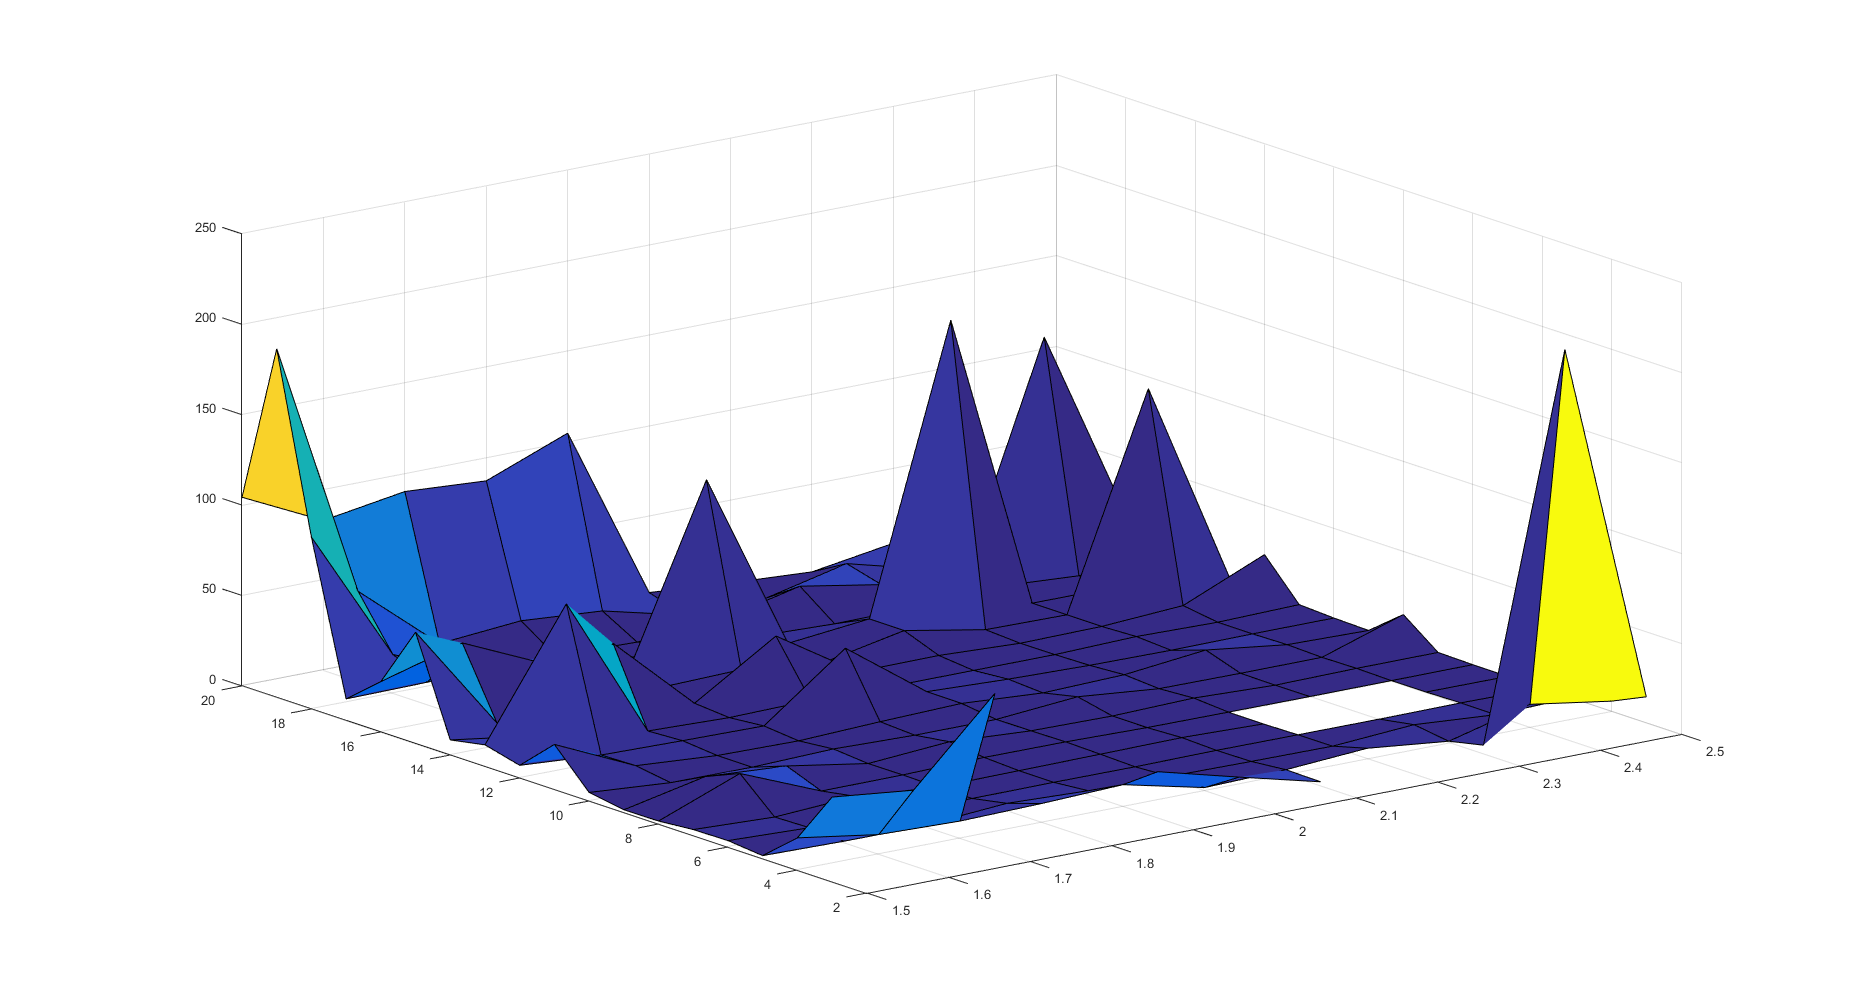
\includegraphics[scale=.3]{dq_kegg.png}
    \caption{Wykres wartości $\left| Q_\text{learn} - Q_\text{test} \right|$ dla zbioru 
        \emph{KEGG Metabolic Relation Network (Undirected)}}
    \label{fig:kegg}
\end{figure}

\subsubsection{Energy efficiency}
Wyniki badań określają efektywność energetyczną, tj. obciążenie cieplne, jako funkcję parametrów budynku.
Zawiera on następujące dane wejściowe:
\begin{itemize}
\item względna zwartość
\item pole powierzchni (całość)
\item pole powierzchni ścian
\item pole powierzchni dachu
\item wysokość
\item orientacja
\item pole powierzchni okien
\item rozmieszczenie okien
\end{itemize}
Na bazie tych parametrów obliczane jest obciążenie cieplne, będące ciągłą wartością zmiennoprzecinkową.
Analiza wykazała, że wskaźnik dopasowania rośnie tylko dla niskich wartości parametru dopasowania $m$ oraz
liczbie klastrów większej od $c = 6$. 

\begin{figure}[h]
    \centering
    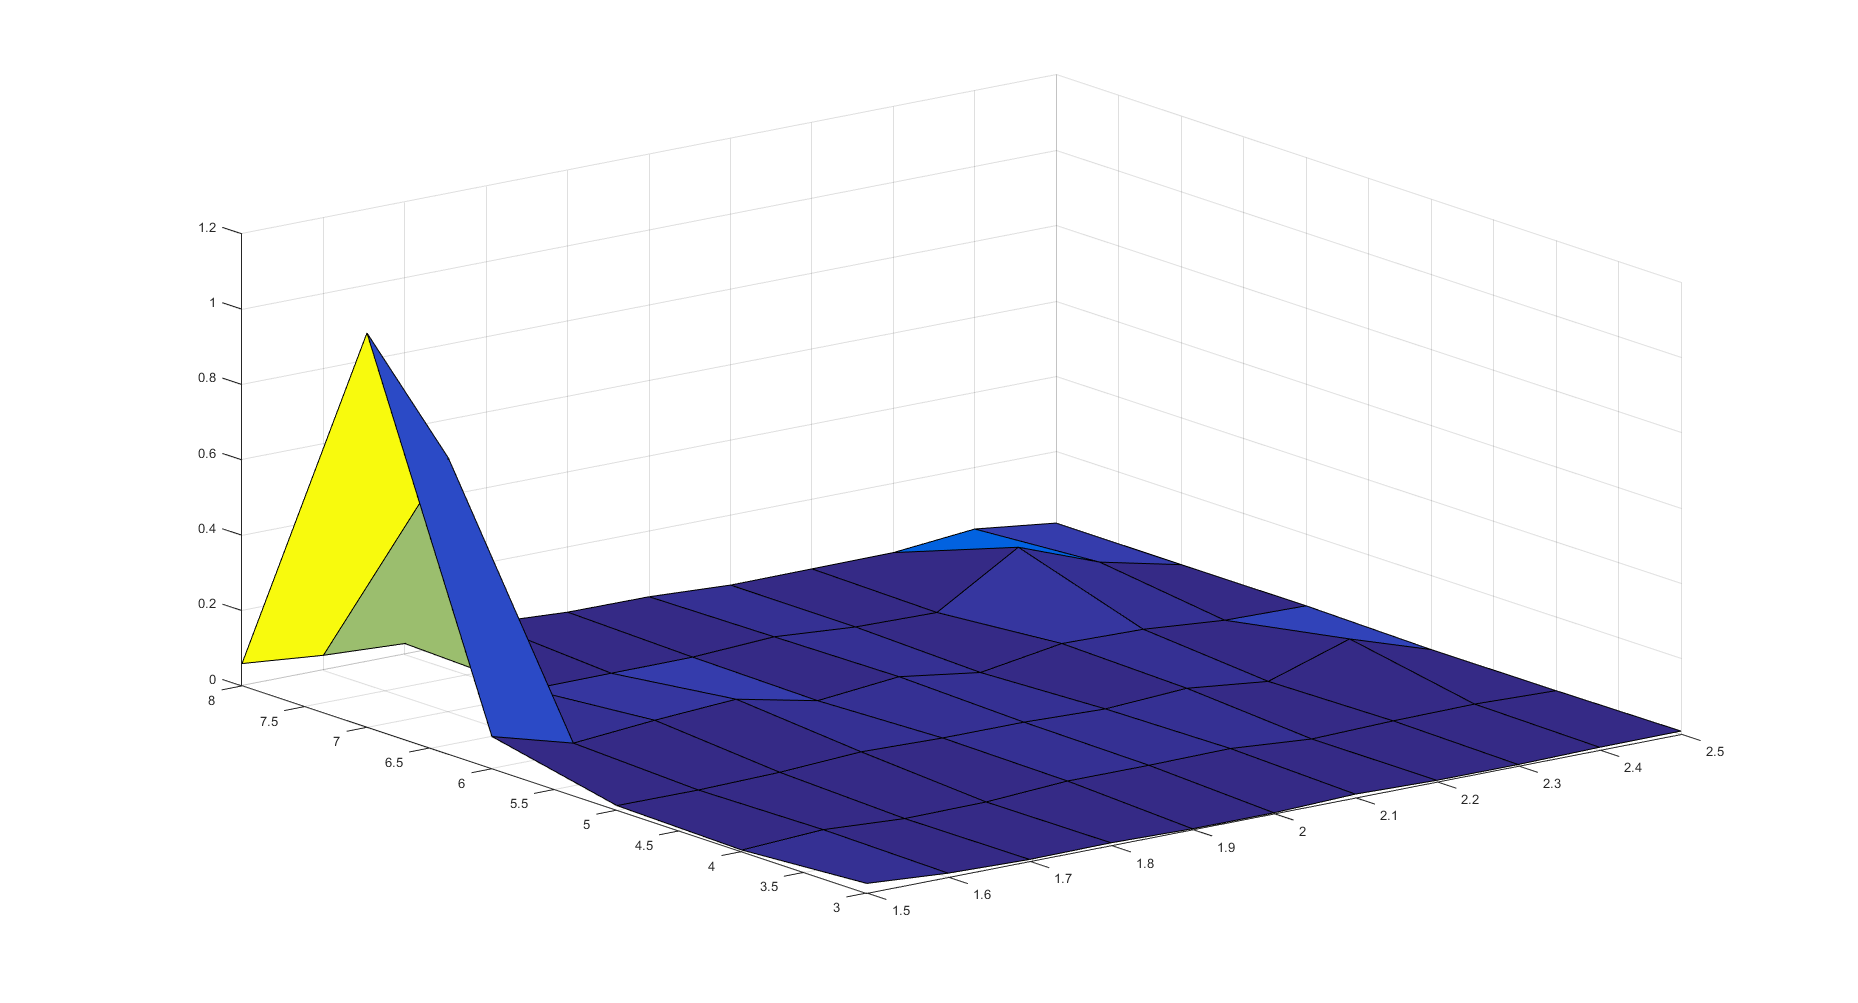
\includegraphics[scale=0.3]{dq_energyeff.png}
    \caption{Wykres wartości $\left| Q_\text{learn} - Q_\text{test} \right|$ dla zbioru 
        \emph{Energy efficiency}}
    \label{fig:ee}
\end{figure}

\subsubsection{Boston housing}
Zbiór danych zawiera wartości nieruchomości na terenach podmiejskich Bostonu. Argumentami są:

\begin{itemize}
\item Współczynnik przestępczości
\item Odsetek parceli mieszkalnych powyżej $2322.5m^2$
\item Odsetek powierzchni przestrzeni biznesowych
\item Wskaźnik Charlesa Rivera
\item Stężenie tlenków węgla
\item Średnia ilość pokoi w mieszkaniu
\item Odsetek zamieszkałych przez właścicieli posiadłości wybudowanych przed 1940r.
\item Średnia ważona odległość do pięciu urzędów pracy
\item Współczynnik dostępności do węzłów autostradowych
\item Wartość podatek od nieruchmości na $\$10000$
\item Współczynnik ilości uczniów do nauczycieli
\item Odsetek ludności czarnoskórej
\item Procent ludności biednej
\item Mediana wartości posiadłości (w $\$1000$)
\end{itemize}

Wartością traktowaną jako wartość funkcji jest mediana wartości posiadłości wyrażona w tysiącach dolarów.

\subsubsection{Auto MPG}
Zbiór danych zawiera dane samochodów oraz ilość spalanego przez nie paliwa w cyklu miejskim. Argumentami są:

\begin{itemize}
\item Ilość cylindrów
\item Objętość skokowa
\item Ilość koni mechanicznych
\item Waga
\item Przyspieszenie
\item Rok produkcji
\item Pochodzenie
\end{itemize}

\begin{figure}[h]
    \centering
    \begin{minipage}{0.45\textwidth}
        \centering
        \resizebox{1.2\textwidth}{!}{\input{w_mpg_learn}}
        \caption{Wykres wartości $Q_\text{learn}$ dla zbioru \emph{Auto MPG}}
        \label{fig:mpg_learn}
    \end{minipage}\hfill
    \begin{minipage}{0.45\textwidth}
        \centering
        \resizebox{1.2\textwidth}{!}{\input{w_mpg_test}}
        \caption{Wykres wartości $Q_\text{test}$ dla zbioru \emph{Auto MPG}}
        \label{fig:mpg_test}
    \end{minipage}
\end{figure}

Wartością funkcji jest spalanie paliwa wyrażone w galonach na milę.

Analiza wartości wskaźników dopasowania $Q$ ukazuje, że zbiór danych nie
charakteryzuje się podziałem na klastry.
Aby utrzymać wartość wskaźnika $Q_\text{test}$ na niewielkim poziomie nie
powinno się wybierać zbyt dużej ilości klastrów, co widać na Rys.~\ref{fig:mpg_test}.
Tak jak w przypadku \emph{Energy Efficiency} przy dzieleniu na dużą ilość klastrów,
przy użyciu niskich wartości parametru $m$, występuje efekt drastycznego pogorszenia $Q$.

\subsection{Wnioski}
Dla zbiorów \emph{Energy efficiency} oraz \emph{Auto MPG} możemy zauważyć bardzo niski wskaźnik $Q$ co sugeruje,
że dane są poprawnie dzielone na klastry i ich odtworzenie nie powinno sprawić problemów. Jedynie przy dużej
(zbliżonej do ilości argumentów) ilości klastrów oraz wartości parametru $m$ ze skrajów testowanych wartości
możemy zauważyć nagły wzrost $Q$.

\section{Podział prac}

\textbf{Marcin Kołodziej} wykonał
\begin{itemize}
\item testy sprawności algorytmu
\item obliczenia sprawności modelu TS dla zbiorów \emph{KEGG Metabolic Relation Network (Undirected)} oraz \emph{Energy efficiency}
\end{itemize}

\textbf{Jakub Sawicki} wykonał
\begin{itemize}
\item implementację FCM i~TS w~MATLAB
\item obliczenia sprawności modelu TS dla zbiorów \emph{Boston housing} oraz \emph{Auto MPG}
\end{itemize}
\end{document}

